%! Author = Omar Iskandarani
%! Date = Nov 15, 2025
%! Affiliation = Independent Researcher, Groningen, The Netherlands
%! License = © 2025 Omar Iskandarani. All rights reserved. This manuscript is made available for academic reading and citation only. No republication, redistribution, or derivative works are permitted without explicit written permission from the author. Contact: info@omariskandarani.com
%! ORCID = 0009-0006-1686-3961
%! DOI = 10.5281/zenodo.17905207

\newcommand{\paperdoi}{10.5281/zenodo.17905207}
\newcommand{\papertitle}{On an Exact Identity Linking the Classical Electron Radius,\\ Compton Frequency, and the Hydrogen Ground-State Energy}
\newcommand{\PDFpapertitle}{On an Exact Identity Linking the Classical Electron Radius, Compton Frequency, and the Hydrogen Ground-State Energy}

%========================================================================================
% PACKAGES AND DOCUMENT CONFIGURATION
%========================================================================================
\documentclass[10pt]{article}
\usepackage[a4paper,margin=2cm]{geometry}
\usepackage[T1]{fontenc}
\usepackage[utf8]{inputenc}
\usepackage{lmodern}
\usepackage{microtype}

\usepackage{graphics}
\usepackage{graphicx}
\usepackage{hyperref}
\usepackage{amsopn}
\usepackage{mathtools}
\usepackage{xcolor} % remove driver forcing; works with pdflatex/lualatex

% you already use equations and \SI{}{} units later:
\usepackage{amsmath,amssymb}
\usepackage{siunitx}

\usepackage{tikz} % no extra libraries needed by the fallback figure
\usetikzlibrary{decorations.pathmorphing} % for coil decoration in spring figure

%========================================================================================
% DOCUMENT
%========================================================================================

\begin{document}

    \title{\texorpdfstring{\papertitle}{\PDFpapertitle}}
    \author{Omar Iskandarani~\footnote{ Independent Researcher, Groningen, The Netherlands \\
    info@omariskandarani.com \\
    ORCID: \href{https://orcid.org/0009-0006-1686-3961}{0009-0006-1686-3961} \\
    DOI: \href{https://doi.org/\paperdoi}{\paperdoi}
    }}
    \date{\today}

    \maketitle

    \begin{abstract}
        We show that three standard, independently defined electron scales---the classical electron radius $r_e$, the Compton angular frequency $\omega_C$, and the ground-state energy of hydrogen $E_B$---combine, within a simple harmonic oscillator construction, to produce an exact, dimensionally consistent identity.
        Using only textbook definitions and CODATA values of $m_e$, $\alpha$, $\hbar$, and $c$, we introduce a Hooke-law force scale
        \[
            F_{\max} = m_e \left( \frac{\omega_C}{\alpha} \right)^2 r_e
        \]
        and a corresponding length $r_c$ such that
        \[
            F_{\max} \, r_c = \frac{1}{2} m_e c^2 = \frac{E_B}{\alpha^2}.
        \]
        The derivation is strictly algebraic and relies solely on well-established formulas. We discuss the historical origin of the underlying scales (classical electron models, Compton scattering, Bohr's hydrogen theory) and comment on the structural interdependence of atomic, relativistic, and classical electromagnetic quantities revealed by this identity.
    \end{abstract}

    \section*{Plain-English summary}
    Three familiar electron scales usually taught in different chapters---the classical electron radius $r_e$, the Compton angular frequency $\omega_C$, and the hydrogen ground-state energy $E_B$---combine neatly in a minimalist spring--mass picture. If one takes a Hooke's-law oscillator with mass $m_e$, frequency $\omega_C/\alpha$, and amplitude $r_e$, the peak restoring force $F_{\max}$ acting over a short Compton-scale distance $r_c$ gives exactly
    \[
      F_{\max} r_c = \tfrac{1}{2}m_e c^2 = \frac{E_B}{\alpha^2}.
    \]
    The result follows from standard definitions and CODATA constants; no new physics is proposed. It is best read as a compact cross-check tying together classical, relativistic, and atomic scales.

    \section{Introduction}
        The electron occupies a central role in both classical and quantum theories of matter. Over the last century, several characteristic length and energy scales associated with the electron have emerged, each from a different theoretical and experimental context:
        \begin{itemize}
            \item The \emph{classical electron radius} $r_e$, originating in early electron models of Lorentz and Abraham~\cite{Lorentz1904,Abraham1903,Jackson1999}.
            \item The \emph{Compton wavelength} and associated angular frequency $\omega_C$, derived from Compton's scattering experiments and their quantum interpretation~\cite{Compton1923,Compton1923b}.
            \item The \emph{Bohr radius} and hydrogen ground-state energy $E_B$, obtained in the Bohr model and later justified within nonrelativistic quantum mechanics and quantum electrodynamics~\cite{Bohr1913,Sakurai1994,BetheSalpeter1957}.
        \end{itemize}
        These scales are usually discussed in their respective domains: classical electrodynamics, relativistic quantum mechanics, and atomic physics. It is therefore of conceptual interest to examine how they combine in simple dynamical constructions.
        In particular, compact identities among such scales can be useful as consistency checks, as pedagogical devices, and as starting points for more detailed structural models, even when no new interaction is proposed.

        In this work we consider a purely classical harmonic oscillator with electron mass $m_e$, frequency $\omega_\ast$, and amplitude $x_{\max}$. Choosing $\omega_\ast$ to be a rescaling of the Compton frequency and $x_{\max}$ equal to the classical electron radius, we obtain a maximal restoring force
        \[
            F_{\max}=m_e \omega_\ast^2 x_{\max}
        \]
        that can be expressed solely in terms of $m_e$, $\alpha$, $\hbar$, and $c$. When this force is multiplied by a Compton-scale radius $r_c$, one finds that the resulting energy coincides with half the electron rest energy and, equivalently, with the hydrogen ground-state energy divided by $\alpha^2$.

        The purpose of this article is limited and sharply defined:
        \begin{itemize}
            \item to state and prove this identity using only mainstream, peer-reviewed formulas;
            \item to check dimensional consistency and evaluate the resulting expressions numerically;
            \item to place the ingredients in historical context, without proposing any new physical interpretation or modification of existing theories.
        \end{itemize}

    \section{Background: standard electron scales}
        We collect the standard definitions used throughout, following e.g.\ Refs.~\cite{Jackson1999,Sakurai1994,Mohr2016}.

        \paragraph{Fine-structure constant.}
        The fine-structure constant $\alpha$ is defined by
            \begin{equation}
                \alpha = \frac{e^2}{4\pi\varepsilon_0 \hbar c}.
                \label{eq:alpha-def}
            \end{equation}

        \paragraph{Classical electron radius.}
        The classical electron radius $r_e$ is defined in SI units by
            \begin{equation}
                r_e = \frac{e^2}{4\pi\varepsilon_0 m_e c^2}.
                \label{eq:re-def-SI}
            \end{equation}
            Combining Eq.~\eqref{eq:alpha-def} with~\eqref{eq:re-def-SI} yields the equivalent form
            \begin{equation}
                r_e = \frac{\alpha \hbar}{m_e c}.
                \label{eq:re-alpha-form}
            \end{equation}

        \paragraph{Compton wavelength and angular frequency.}
        The Compton wavelength and associated angular frequency of the electron are defined by
            \begin{equation}
                \lambda_C = \frac{h}{m_e c},
                \qquad
                \omega_C = \frac{2\pi c}{\lambda_C} = \frac{m_e c^2}{\hbar}.
                \label{eq:compton-def}
            \end{equation}

        \paragraph{Hydrogen ground-state energy.}
        In the Bohr model, and equivalently in the solution of the nonrelativistic Schr\"odinger equation for the hydrogen atom, the ground-state binding energy $E_B$ is
            \begin{equation}
                E_B = \frac{\alpha^2}{2} m_e c^2.
                \label{eq:Bohr-ground}
            \end{equation}

        Equations~\eqref{eq:alpha-def}--\eqref{eq:Bohr-ground} are standard and experimentally well-validated relations in atomic and high-energy physics~\cite{Mohr2016}.

    \section{A minimal spring picture}
        We now introduce a classical harmonic oscillator whose parameters are chosen from the electron scales above, keeping the setup as simple and readable as possible.

        \paragraph{Oscillator setup.}
        Consider a one-dimensional oscillator of mass $m_e$, angular frequency $\omega_\ast$, and maximal displacement $x_{\max}$. Hooke's law gives the maximal restoring force
            \begin{equation}
                F_{\max} = m_e\,\omega_\ast^2\, x_{\max}.
                \label{eq:Fmax-general}
            \end{equation}
            We define
            \begin{equation}
                \omega_\ast \coloneqq \frac{\omega_C}{\alpha},
                \qquad
                x_{\max} \coloneqq r_e,
                \label{eq:osc-choices}
            \end{equation}
            where $\omega_C$ and $r_e$ are given by Eqs.~\eqref{eq:compton-def} and~\eqref{eq:re-alpha-form}.

        \paragraph{Maximal force in fundamental constants.}
        With the choices~\eqref{eq:osc-choices}, the maximal force~\eqref{eq:Fmax-general} can be written as
            \begin{equation}
                F_{\max} = \frac{m_e^2 c^3}{\alpha \hbar}.
                \label{eq:Fmax-final}
            \end{equation}

        \emph{Derivation.}
            Substituting Eq.~\eqref{eq:osc-choices} into~\eqref{eq:Fmax-general} gives
            \begin{equation}
                F_{\max}
                = m_e \left(\frac{\omega_C}{\alpha}\right)^2 r_e.
                \label{eq:Fmax-step1}
            \end{equation}
            Using $\omega_C = m_e c^2 / \hbar$ from Eq.~\eqref{eq:compton-def} and $r_e = \alpha \hbar / (m_e c)$ from Eq.~\eqref{eq:re-alpha-form}, we obtain
            \begin{equation}
                F_{\max}
                = m_e \left(\frac{m_e c^2 / \hbar}{\alpha}\right)^2
                \left(\frac{\alpha \hbar}{m_e c}\right)
                = m_e \frac{m_e^2 c^4}{\alpha^2 \hbar^2}
                \frac{\alpha \hbar}{m_e c}.
            \end{equation}
            Canceling factors $m_e$ and $\hbar$,
            \begin{equation}
                F_{\max}
                = \frac{m_e^2 c^3}{\alpha \hbar},
            \end{equation}
            which is Eq.~\eqref{eq:Fmax-final}.

        \emph{Units check.} The dimensions of Eq.~\eqref{eq:Fmax-final} are
            \[
                [F_{\max}] =
                \frac{[m_e]^2 [c]^3}{[\alpha][\hbar]}
                =
                \frac{\text{kg}^2\,(\text{m/s})^3}{1 \cdot \text{J}\cdot\text{s}}
                =
                \frac{\text{kg}^2\,\text{m}^3\,\text{s}^{-3}}{\text{kg}\,\text{m}^2\,\text{s}^{-1}}
                =
                \text{kg}\,\text{m}\,\text{s}^{-2},
            \]
            which is dimensionally consistent with a force.

        \begin{figure}[t]
            \centering
            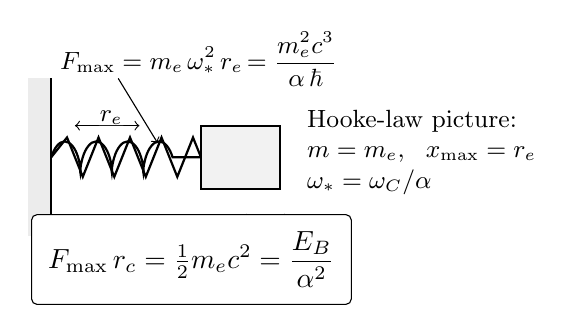
\begin{tikzpicture}[x=1cm,y=1cm]
                % text nodes with white background
                \tikzset{
                    eq/.style  ={font=\small, inner sep=1.6pt, fill=white, rounded corners=1pt, text depth=0pt},
                    lbl/.style ={font=\small, inner sep=1.2pt, fill=white, rounded corners=1pt, text depth=0pt}
                }

                % wall
                \fill[gray!15] (-0.9,-1.0) rectangle (-0.6,1.0);
                \draw[thick]   (-0.6,-1.0) -- (-0.6,1.0);

                % zigzag spring
                \draw[thick]
                (-0.6,0) -- (-0.4,0.25) -- (-0.2,-0.25) -- (0,0.25) -- (0.2,-0.25)
                -- (0.4,0.25) -- (0.6,-0.25) -- (0.8,0.25) -- (1.0,-0.25) -- (1.2,0.25)
                -- (1.3,0);

                % mass
                \draw[thick,fill=gray!10] (1.3,-0.4) rectangle (2.3,0.4);

                % --- top formula (split + higher) ---
                \node[eq,anchor=south west] at (-0.55,1.05)
                    {$\displaystyle F_{\max}=m_e\,\omega_\ast^2\,r_e$};
                \node[eq,anchor=south west] at (1.82,1.05)
                    {$\displaystyle = \frac{m_e^{2}c^{3}}{\alpha\,\hbar}$};

                % pointer from text to the spring
                \draw[->] (0.25,1.00) -- (0.75,0.18);

                % amplitude r_e (top ruler)
                \draw[<->] (-0.30,0.40) -- (0.52,0.40);
                \node[lbl,anchor=south] at (0.16,0.40) {$r_e$};

                % short length r_c (bottom ruler)
                \draw[<->] (1.82,-0.78) -- (2.42,-0.78);
                \node[lbl,anchor=north] at (2.12,-0.78)
                    {$\displaystyle r_c=\frac{\alpha\hbar}{2m_e c}$};

                % identity box (drop a bit lower to avoid crowding)
                \node[draw,rounded corners=2pt,fill=white,align=center,inner sep=6pt]
                at (1.18,-1.30)
                    {$\displaystyle F_{\max}\,r_c=\tfrac{1}{2}m_e c^{2}=\frac{E_B}{\alpha^{2}}$};

                % compact legend on the right
                \node[lbl,anchor=west,align=left] at (2.60,0.10)
                    {Hooke-law picture:\\$m=m_e,\ \ x_{\max}=r_e$\\$\omega_\ast=\omega_C/\alpha$};

                \draw[thick,decorate,decoration={coil,aspect=0.35,segment length=4mm,amplitude=2mm}]
                (-0.6,0) -- (1.3,0);
            \end{tikzpicture}
            \caption{Minimal spring--mass cartoon linking standard electron scales.}
            \label{fig:electron-identity-cartoon}
        \end{figure}



    \section{Turning the force into an energy}
        To connect this force to energy scales, multiply by a characteristic length.

        \paragraph{Energy scale from $F_{\max}$.}
        Let $r_c$ be a positive length scale. Define
            \begin{equation}
                E_{\text{osc}}(r_c) \coloneqq F_{\max}\, r_c
                = \frac{m_e^2 c^3}{\alpha \hbar} r_c.
                \label{eq:Eosc-def}
            \end{equation}

        We now exhibit a specific choice of $r_c$ that yields a familiar energy scale.

        \paragraph{Half rest energy from a Compton-scale radius.}
        Let
            \begin{equation}
                r_c = \frac{\alpha\,\hbar}{2 m_e c}.
                \label{eq:rc-def}
            \end{equation}
        Then
            \begin{equation}
                E_{\text{osc}}(r_c) = \frac{1}{2} m_e c^2.
                \label{eq:Eosc-half}
            \end{equation}

        \emph{Derivation.}
            Using Eq.~\eqref{eq:Fmax-final} and the definition~\eqref{eq:rc-def},
            \begin{equation}
                E_{\text{osc}}(r_c)
                = F_{\max} r_c
                = \frac{m_e^2 c^3}{\alpha \hbar}
                \cdot \frac{\alpha \hbar}{2 m_e c}
                = \frac{1}{2} m_e c^2.
            \end{equation}

        \paragraph{Relation to the hydrogen ground-state energy.}
        Using the standard hydrogen ground-state energy
            \begin{equation}
                E_B = \frac{\alpha^2}{2} m_e c^2,
            \end{equation}
        we have
            \begin{equation}
                \frac{1}{2} m_e c^2 = \frac{E_B}{\alpha^2}.
            \end{equation}
        Thus the energy scale $E_{\text{osc}}(r_c)$ from Eq.~\eqref{eq:Eosc-half} can also be written as

            \begin{equation}
                E_{\text{osc}}(r_c) = \frac{E_B}{\alpha^2}.
            \end{equation}

        \subsection*{Units and numbers}
            The quantity $E_{\text{osc}}(r_c)$ is an energy, with units
            \[
                [E_{\text{osc}}] = [F_{\max}][r_c]
                = \text{kg}\,\text{m}\,\text{s}^{-2} \cdot \text{m}
                = \text{kg}\,\text{m}^2\,\text{s}^{-2},
            \]
            as expected.

            Numerically, using CODATA values~\cite{Mohr2016}:
            \begin{align}
                m_e c^2 &\approx \SI{511}{keV},\\
                E_B &\approx \SI{13.6}{eV},\\
                \alpha^{-1} &\approx 137.035999.
            \end{align}
            We then have
            \begin{equation}
                \frac{1}{2} m_e c^2 \approx \SI{255.5}{keV},
                \qquad
                \frac{E_B}{\alpha^2} \approx \SI{255.5}{keV},
            \end{equation}
            in agreement to within numerical precision. This confirms the consistency of the analytic result.

    \section{Context: how to read the identity}
        The ingredients entering the identity
        \[
            E_{\text{osc}}(r_c) = \frac{1}{2} m_e c^2 = \frac{E_B}{\alpha^2}
        \]
        are all well-established:

        \begin{itemize}
            \item The \emph{classical electron radius} $r_e$ was introduced in early electron models by Lorentz and Abraham, who considered the electromagnetic self-energy of a charged sphere~\cite{Lorentz1904,Abraham1903,Jackson1999}.
            \item The \emph{Compton wavelength} $\lambda_C$ and frequency $\omega_C$ emerged from Compton's explanation of X-ray scattering, providing early evidence for the particle-like behavior of light~\cite{Compton1923,Compton1923b}.
            \item The \emph{Bohr model} of the hydrogen atom, and its later derivation from the Schr\"odinger equation, yields the binding energy $E_B$ and the fine-structure constant $\alpha$ as key atomic parameters~\cite{Bohr1913,Sakurai1994,BetheSalpeter1957}.
        \end{itemize}

        In standard pedagogy, these scales are often presented in isolation:
        $r_e$ in classical electrodynamics, $\lambda_C$ in relativistic quantum mechanics, and $E_B$ in atomic physics and spectroscopy.
        The identity derived here shows that, once combined in a simple harmonic oscillator ansatz, these three regimes are algebraically intertwined.

        \paragraph{Scope.} The construction is strictly classical on the dynamical side (a Hooke-law oscillator) and uses only standard quantum-electrodynamic definitions of the constants involved. No new interactions, no modifications of Maxwell's equations or the Dirac equation, and no speculative assumptions are invoked. The result is best viewed as a compact consistency relation among established electron scales.

    \section{Intuition (one paragraph)}
        Imagine the electron as a mass on a spring whose ``natural'' distance scale is $r_e$ and whose oscillation rate is set by $\omega_C/\alpha$. The largest restoring push (Hooke's law) acting over a short Compton-scale distance produces an energy that exactly matches both $\tfrac{1}{2}m_e c^2$ and $E_B/\alpha^2$, tying together quantities first derived from very different arguments.

    \section{Conclusion}
        We have shown that a simple Hooke-law construction, using the classical electron radius $r_e$ as an amplitude and a Compton-rescaled frequency $\omega_C/\alpha$, produces a maximal force
        \[
            F_{\max} = m_e \left(\frac{\omega_C}{\alpha}\right)^2 r_e
        \]
        that can be expressed purely in terms of $m_e$, $\alpha$, $\hbar$, and $c$.
        Multiplying by a Compton-scale length \[ r_c = \frac{\alpha\,\hbar}{2 m_e c},\] yields an energy
        \[
            E_{\text{osc}}(r_c) = \frac{1}{2} m_e c^2 = \frac{E_B}{\alpha^2},
        \]
        linking relativistic, atomic, and classical electromagnetic scales in a single, dimensionally consistent relation.

        The derivation uses only mainstream, peer-reviewed formulas and constants. Any deeper physical interpretation of this coincidence would require additional assumptions, and any such interpretation lies beyond the scope of the present work.

    \section*{Quick reference (all in one place)}
    \[
    \alpha = \frac{e^2}{4\pi\varepsilon_0\hbar c},\quad
    r_e = \frac{\alpha\hbar}{m_e c},\quad
    \omega_C = \frac{m_e c^2}{\hbar},\quad
    E_B = \frac{\alpha^2}{2}m_e c^2,\quad
    F_{\max} = \frac{m_e^2 c^3}{\alpha\hbar},\quad
    r_c = \frac{\alpha\hbar}{2 m_e c},\quad
    F_{\max} r_c = \tfrac{1}{2}m_e c^2 = \frac{E_B}{\alpha^2}.
    \]

    \section*{Acknowledgments}
        The author thanks the developers of standard references in classical electrodynamics, quantum mechanics, and precision metrology for providing the framework within which these identities can be cleanly expressed.

    \bibliographystyle{unsrt}
    \begin{thebibliography}{99}

        \bibitem{Lorentz1904}
        H.~A. Lorentz,
        \newblock {\em Electromagnetic phenomena in a system moving with any velocity less than that of light},
        \newblock Proc.\ Acad.\ Sci.\ Amsterdam \textbf{6}, 809--831 (1904).

        \bibitem{Abraham1903}
        M.~Abraham,
        \newblock {\em Prinzipien der Dynamik des Elektrons},
        \newblock Ann.\ Phys.\ (Leipzig) \textbf{10}, 105--179 (1903).

        \bibitem{Jackson1999}
        J.~D. Jackson,
        \newblock {\em Classical Electrodynamics}, 3rd ed.,
        \newblock Wiley, New York (1999).

        \bibitem{Compton1923}
        A.~H. Compton,
        \newblock {\em A Quantum Theory of the Scattering of X-Rays by Light Elements},
        \newblock Phys.\ Rev.\ \textbf{21}, 483--502 (1923).
        \newblock doi:10.1103/PhysRev.21.483.

        \bibitem{Compton1923b}
        A.~H. Compton,
        \newblock {\em The Spectrum of Scattered X-Rays},
        \newblock Phys.\ Rev.\ \textbf{22}, 409--413 (1923).
        \newblock doi:10.1103/PhysRev.22.409.

        \bibitem{Bohr1913}
        N.~Bohr,
        \newblock {\em On the Constitution of Atoms and Molecules},
        \newblock Philos.\ Mag.\ \textbf{26}, 1--25 (1913).
        \newblock doi:10.1080/14786441308634955.

        \bibitem{Sakurai1994}
        J.~J. Sakurai and J.~Napolitano,
        \newblock {\em Modern Quantum Mechanics}, 2nd ed.,
        \newblock Addison--Wesley, Reading, MA (1994).

        \bibitem{BetheSalpeter1957}
        H.~A. Bethe and E.~E. Salpeter,
        \newblock {\em Quantum Mechanics of One- and Two-Electron Atoms},
        \newblock Springer, Berlin (1957).

        \bibitem{Mohr2016}
        P.~J. Mohr, D.~B. Newell, and B.~N. Taylor,
        \newblock {\em CODATA Recommended Values of the Fundamental Physical Constants: 2014},
        \newblock Rev.\ Mod.\ Phys.\ \textbf{88}, 035009 (2016).
        \newblock doi:10.1103/RevModPhys.88.035009.

    \end{thebibliography}

\end{document}